\begin{figure*}[ht]\centering
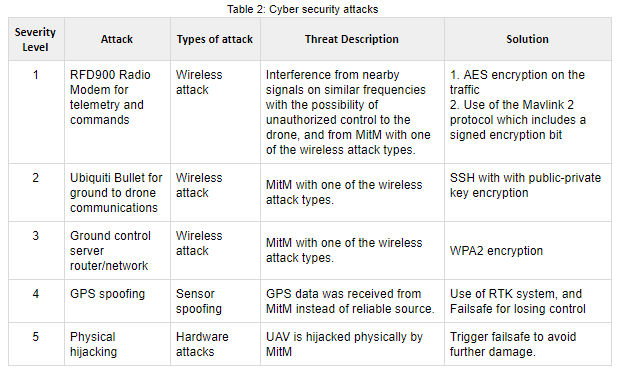
\includegraphics[width=0.8\textwidth]{table/Table_2_cyber_security_attacks.PNG}
\caption*{}
\label{fig:cs}
\end{figure*}
The UAS system is vulnerable to three types of attacks: hardware attacks, wireless attacks and sensor spoofing. 

Hardware attacks includes attacks where man-in-the-middle (MitM) directly attacks the components of the UAV, such as physically hijacking the UAV. Wireless attacks are when the attacker intercepts, modifies, fabricates identity or denies of service (DoS) the communicate links or nodes. Sensor spoofing is when attackers interrupt the UAV’s on-board sensor data.



The team enhanced the security of its system by adding multiple layers of protection to prevent threats from different aspects. Table 2 illustrates four major security threats with their severity level identified (1 being the highest) within the current system design and solutions the team has implemented. The main focus has been to address Wireless attacks. See table 2.



% \onecolumn
% \begin{table}[t]
%     \centering
%     \normalsize
%     \label{tab:cyber_security}

%     \begin{tabular}{p{1cm} p{4cm} p{3cm} p{5cm} p{5cm}}
%     \hline
%     Severity Level & Attack & Types of attack & Threat description & Solution \\ 
%     \hline
%     1&RFD900 Radio Modem for telemetry and commands&Wireless attack&
%     Interference from nearby signals on similar frequencies with the possibility of unauthorized control to the drone, and from MitM with one of the wireless attack types. 
%     & \begin{enumerate}
%         \item AES encryption on the traffic \item Use of the Mavlink 2 protocol which includes a signed encryption bit
%     \end{enumerate} \\ 
    
%     \hline
%     2&Ubiquiti Bullet for ground to drone communications&Wireless attack&MitM with one of the wireless attack types. & SSH with with public-private key encryption \\
%     \hline
%     3&Ground control server router/network&Wireless attack& MitM with one of the wireless attack types. &WPA2 encryption \\
%     \hline
%     4&GPS spoofing& Sensor spoofing&GPS data was received from MitM instead of reliable source. & Use of RTK system, and Failsafe for losing control\\
%     \hline
%     5&
%     Physical hijacking &Hardware attacks&UAV is hijacked physically by MitM&Trigger failsafe to avoid further damage.  \\
     
%     \end{tabular}
% \end{table}
% \twocolumn

\endinput